\documentclass[11pt]{article}

    \usepackage[breakable]{tcolorbox}
    \usepackage{parskip} % Stop auto-indenting (to mimic markdown behaviour)
    
    \usepackage{iftex}
    \ifPDFTeX
    	\usepackage[T1]{fontenc}
    	\usepackage{mathpazo}
    \else
    	\usepackage{fontspec}
    \fi

    % Basic figure setup, for now with no caption control since it's done
    % automatically by Pandoc (which extracts ![](path) syntax from Markdown).
    \usepackage{graphicx}
    % Maintain compatibility with old templates. Remove in nbconvert 6.0
    \let\Oldincludegraphics\includegraphics
    % Ensure that by default, figures have no caption (until we provide a
    % proper Figure object with a Caption API and a way to capture that
    % in the conversion process - todo).
    \usepackage{caption}
    \DeclareCaptionFormat{nocaption}{}
    \captionsetup{format=nocaption,aboveskip=0pt,belowskip=0pt}

    \usepackage[Export]{adjustbox} % Used to constrain images to a maximum size
    \adjustboxset{max size={0.9\linewidth}{0.9\paperheight}}
    \usepackage{float}
    \floatplacement{figure}{H} % forces figures to be placed at the correct location
    \usepackage{xcolor} % Allow colors to be defined
    \usepackage{enumerate} % Needed for markdown enumerations to work
    \usepackage{geometry} % Used to adjust the document margins
    \usepackage{amsmath} % Equations
    \usepackage{amssymb} % Equations
    \usepackage{textcomp} % defines textquotesingle
    % Hack from http://tex.stackexchange.com/a/47451/13684:
    \AtBeginDocument{%
        \def\PYZsq{\textquotesingle}% Upright quotes in Pygmentized code
    }
    \usepackage{upquote} % Upright quotes for verbatim code
    \usepackage{eurosym} % defines \euro
    \usepackage[mathletters]{ucs} % Extended unicode (utf-8) support
    \usepackage{fancyvrb} % verbatim replacement that allows latex
    \usepackage{grffile} % extends the file name processing of package graphics 
                         % to support a larger range
    \makeatletter % fix for grffile with XeLaTeX
    \def\Gread@@xetex#1{%
      \IfFileExists{"\Gin@base".bb}%
      {\Gread@eps{\Gin@base.bb}}%
      {\Gread@@xetex@aux#1}%
    }
    \makeatother

    % The hyperref package gives us a pdf with properly built
    % internal navigation ('pdf bookmarks' for the table of contents,
    % internal cross-reference links, web links for URLs, etc.)
    \usepackage{hyperref}
    % The default LaTeX title has an obnoxious amount of whitespace. By default,
    % titling removes some of it. It also provides customization options.
    \usepackage{titling}
    \usepackage{longtable} % longtable support required by pandoc >1.10
    \usepackage{booktabs}  % table support for pandoc > 1.12.2
    \usepackage[inline]{enumitem} % IRkernel/repr support (it uses the enumerate* environment)
    \usepackage[normalem]{ulem} % ulem is needed to support strikethroughs (\sout)
                                % normalem makes italics be italics, not underlines
    \usepackage{mathrsfs}
    

    
    % Colors for the hyperref package
    \definecolor{urlcolor}{rgb}{0,.145,.698}
    \definecolor{linkcolor}{rgb}{.71,0.21,0.01}
    \definecolor{citecolor}{rgb}{.12,.54,.11}

    % ANSI colors
    \definecolor{ansi-black}{HTML}{3E424D}
    \definecolor{ansi-black-intense}{HTML}{282C36}
    \definecolor{ansi-red}{HTML}{E75C58}
    \definecolor{ansi-red-intense}{HTML}{B22B31}
    \definecolor{ansi-green}{HTML}{00A250}
    \definecolor{ansi-green-intense}{HTML}{007427}
    \definecolor{ansi-yellow}{HTML}{DDB62B}
    \definecolor{ansi-yellow-intense}{HTML}{B27D12}
    \definecolor{ansi-blue}{HTML}{208FFB}
    \definecolor{ansi-blue-intense}{HTML}{0065CA}
    \definecolor{ansi-magenta}{HTML}{D160C4}
    \definecolor{ansi-magenta-intense}{HTML}{A03196}
    \definecolor{ansi-cyan}{HTML}{60C6C8}
    \definecolor{ansi-cyan-intense}{HTML}{258F8F}
    \definecolor{ansi-white}{HTML}{C5C1B4}
    \definecolor{ansi-white-intense}{HTML}{A1A6B2}
    \definecolor{ansi-default-inverse-fg}{HTML}{FFFFFF}
    \definecolor{ansi-default-inverse-bg}{HTML}{000000}

    % commands and environments needed by pandoc snippets
    % extracted from the output of `pandoc -s`
    \providecommand{\tightlist}{%
      \setlength{\itemsep}{0pt}\setlength{\parskip}{0pt}}
    \DefineVerbatimEnvironment{Highlighting}{Verbatim}{commandchars=\\\{\}}
    % Add ',fontsize=\small' for more characters per line
    \newenvironment{Shaded}{}{}
    \newcommand{\KeywordTok}[1]{\textcolor[rgb]{0.00,0.44,0.13}{\textbf{{#1}}}}
    \newcommand{\DataTypeTok}[1]{\textcolor[rgb]{0.56,0.13,0.00}{{#1}}}
    \newcommand{\DecValTok}[1]{\textcolor[rgb]{0.25,0.63,0.44}{{#1}}}
    \newcommand{\BaseNTok}[1]{\textcolor[rgb]{0.25,0.63,0.44}{{#1}}}
    \newcommand{\FloatTok}[1]{\textcolor[rgb]{0.25,0.63,0.44}{{#1}}}
    \newcommand{\CharTok}[1]{\textcolor[rgb]{0.25,0.44,0.63}{{#1}}}
    \newcommand{\StringTok}[1]{\textcolor[rgb]{0.25,0.44,0.63}{{#1}}}
    \newcommand{\CommentTok}[1]{\textcolor[rgb]{0.38,0.63,0.69}{\textit{{#1}}}}
    \newcommand{\OtherTok}[1]{\textcolor[rgb]{0.00,0.44,0.13}{{#1}}}
    \newcommand{\AlertTok}[1]{\textcolor[rgb]{1.00,0.00,0.00}{\textbf{{#1}}}}
    \newcommand{\FunctionTok}[1]{\textcolor[rgb]{0.02,0.16,0.49}{{#1}}}
    \newcommand{\RegionMarkerTok}[1]{{#1}}
    \newcommand{\ErrorTok}[1]{\textcolor[rgb]{1.00,0.00,0.00}{\textbf{{#1}}}}
    \newcommand{\NormalTok}[1]{{#1}}
    
    % Additional commands for more recent versions of Pandoc
    \newcommand{\ConstantTok}[1]{\textcolor[rgb]{0.53,0.00,0.00}{{#1}}}
    \newcommand{\SpecialCharTok}[1]{\textcolor[rgb]{0.25,0.44,0.63}{{#1}}}
    \newcommand{\VerbatimStringTok}[1]{\textcolor[rgb]{0.25,0.44,0.63}{{#1}}}
    \newcommand{\SpecialStringTok}[1]{\textcolor[rgb]{0.73,0.40,0.53}{{#1}}}
    \newcommand{\ImportTok}[1]{{#1}}
    \newcommand{\DocumentationTok}[1]{\textcolor[rgb]{0.73,0.13,0.13}{\textit{{#1}}}}
    \newcommand{\AnnotationTok}[1]{\textcolor[rgb]{0.38,0.63,0.69}{\textbf{\textit{{#1}}}}}
    \newcommand{\CommentVarTok}[1]{\textcolor[rgb]{0.38,0.63,0.69}{\textbf{\textit{{#1}}}}}
    \newcommand{\VariableTok}[1]{\textcolor[rgb]{0.10,0.09,0.49}{{#1}}}
    \newcommand{\ControlFlowTok}[1]{\textcolor[rgb]{0.00,0.44,0.13}{\textbf{{#1}}}}
    \newcommand{\OperatorTok}[1]{\textcolor[rgb]{0.40,0.40,0.40}{{#1}}}
    \newcommand{\BuiltInTok}[1]{{#1}}
    \newcommand{\ExtensionTok}[1]{{#1}}
    \newcommand{\PreprocessorTok}[1]{\textcolor[rgb]{0.74,0.48,0.00}{{#1}}}
    \newcommand{\AttributeTok}[1]{\textcolor[rgb]{0.49,0.56,0.16}{{#1}}}
    \newcommand{\InformationTok}[1]{\textcolor[rgb]{0.38,0.63,0.69}{\textbf{\textit{{#1}}}}}
    \newcommand{\WarningTok}[1]{\textcolor[rgb]{0.38,0.63,0.69}{\textbf{\textit{{#1}}}}}
    
    
    % Define a nice break command that doesn't care if a line doesn't already
    % exist.
    \def\br{\hspace*{\fill} \\* }
    % Math Jax compatibility definitions
    \def\gt{>}
    \def\lt{<}
    \let\Oldtex\TeX
    \let\Oldlatex\LaTeX
    \renewcommand{\TeX}{\textrm{\Oldtex}}
    \renewcommand{\LaTeX}{\textrm{\Oldlatex}}
    % Document parameters
    % Document title
    \title{Day I - Part III - Introduction to git}
    
    
    
    
    
% Pygments definitions
\makeatletter
\def\PY@reset{\let\PY@it=\relax \let\PY@bf=\relax%
    \let\PY@ul=\relax \let\PY@tc=\relax%
    \let\PY@bc=\relax \let\PY@ff=\relax}
\def\PY@tok#1{\csname PY@tok@#1\endcsname}
\def\PY@toks#1+{\ifx\relax#1\empty\else%
    \PY@tok{#1}\expandafter\PY@toks\fi}
\def\PY@do#1{\PY@bc{\PY@tc{\PY@ul{%
    \PY@it{\PY@bf{\PY@ff{#1}}}}}}}
\def\PY#1#2{\PY@reset\PY@toks#1+\relax+\PY@do{#2}}

\expandafter\def\csname PY@tok@w\endcsname{\def\PY@tc##1{\textcolor[rgb]{0.73,0.73,0.73}{##1}}}
\expandafter\def\csname PY@tok@c\endcsname{\let\PY@it=\textit\def\PY@tc##1{\textcolor[rgb]{0.25,0.50,0.50}{##1}}}
\expandafter\def\csname PY@tok@cp\endcsname{\def\PY@tc##1{\textcolor[rgb]{0.74,0.48,0.00}{##1}}}
\expandafter\def\csname PY@tok@k\endcsname{\let\PY@bf=\textbf\def\PY@tc##1{\textcolor[rgb]{0.00,0.50,0.00}{##1}}}
\expandafter\def\csname PY@tok@kp\endcsname{\def\PY@tc##1{\textcolor[rgb]{0.00,0.50,0.00}{##1}}}
\expandafter\def\csname PY@tok@kt\endcsname{\def\PY@tc##1{\textcolor[rgb]{0.69,0.00,0.25}{##1}}}
\expandafter\def\csname PY@tok@o\endcsname{\def\PY@tc##1{\textcolor[rgb]{0.40,0.40,0.40}{##1}}}
\expandafter\def\csname PY@tok@ow\endcsname{\let\PY@bf=\textbf\def\PY@tc##1{\textcolor[rgb]{0.67,0.13,1.00}{##1}}}
\expandafter\def\csname PY@tok@nb\endcsname{\def\PY@tc##1{\textcolor[rgb]{0.00,0.50,0.00}{##1}}}
\expandafter\def\csname PY@tok@nf\endcsname{\def\PY@tc##1{\textcolor[rgb]{0.00,0.00,1.00}{##1}}}
\expandafter\def\csname PY@tok@nc\endcsname{\let\PY@bf=\textbf\def\PY@tc##1{\textcolor[rgb]{0.00,0.00,1.00}{##1}}}
\expandafter\def\csname PY@tok@nn\endcsname{\let\PY@bf=\textbf\def\PY@tc##1{\textcolor[rgb]{0.00,0.00,1.00}{##1}}}
\expandafter\def\csname PY@tok@ne\endcsname{\let\PY@bf=\textbf\def\PY@tc##1{\textcolor[rgb]{0.82,0.25,0.23}{##1}}}
\expandafter\def\csname PY@tok@nv\endcsname{\def\PY@tc##1{\textcolor[rgb]{0.10,0.09,0.49}{##1}}}
\expandafter\def\csname PY@tok@no\endcsname{\def\PY@tc##1{\textcolor[rgb]{0.53,0.00,0.00}{##1}}}
\expandafter\def\csname PY@tok@nl\endcsname{\def\PY@tc##1{\textcolor[rgb]{0.63,0.63,0.00}{##1}}}
\expandafter\def\csname PY@tok@ni\endcsname{\let\PY@bf=\textbf\def\PY@tc##1{\textcolor[rgb]{0.60,0.60,0.60}{##1}}}
\expandafter\def\csname PY@tok@na\endcsname{\def\PY@tc##1{\textcolor[rgb]{0.49,0.56,0.16}{##1}}}
\expandafter\def\csname PY@tok@nt\endcsname{\let\PY@bf=\textbf\def\PY@tc##1{\textcolor[rgb]{0.00,0.50,0.00}{##1}}}
\expandafter\def\csname PY@tok@nd\endcsname{\def\PY@tc##1{\textcolor[rgb]{0.67,0.13,1.00}{##1}}}
\expandafter\def\csname PY@tok@s\endcsname{\def\PY@tc##1{\textcolor[rgb]{0.73,0.13,0.13}{##1}}}
\expandafter\def\csname PY@tok@sd\endcsname{\let\PY@it=\textit\def\PY@tc##1{\textcolor[rgb]{0.73,0.13,0.13}{##1}}}
\expandafter\def\csname PY@tok@si\endcsname{\let\PY@bf=\textbf\def\PY@tc##1{\textcolor[rgb]{0.73,0.40,0.53}{##1}}}
\expandafter\def\csname PY@tok@se\endcsname{\let\PY@bf=\textbf\def\PY@tc##1{\textcolor[rgb]{0.73,0.40,0.13}{##1}}}
\expandafter\def\csname PY@tok@sr\endcsname{\def\PY@tc##1{\textcolor[rgb]{0.73,0.40,0.53}{##1}}}
\expandafter\def\csname PY@tok@ss\endcsname{\def\PY@tc##1{\textcolor[rgb]{0.10,0.09,0.49}{##1}}}
\expandafter\def\csname PY@tok@sx\endcsname{\def\PY@tc##1{\textcolor[rgb]{0.00,0.50,0.00}{##1}}}
\expandafter\def\csname PY@tok@m\endcsname{\def\PY@tc##1{\textcolor[rgb]{0.40,0.40,0.40}{##1}}}
\expandafter\def\csname PY@tok@gh\endcsname{\let\PY@bf=\textbf\def\PY@tc##1{\textcolor[rgb]{0.00,0.00,0.50}{##1}}}
\expandafter\def\csname PY@tok@gu\endcsname{\let\PY@bf=\textbf\def\PY@tc##1{\textcolor[rgb]{0.50,0.00,0.50}{##1}}}
\expandafter\def\csname PY@tok@gd\endcsname{\def\PY@tc##1{\textcolor[rgb]{0.63,0.00,0.00}{##1}}}
\expandafter\def\csname PY@tok@gi\endcsname{\def\PY@tc##1{\textcolor[rgb]{0.00,0.63,0.00}{##1}}}
\expandafter\def\csname PY@tok@gr\endcsname{\def\PY@tc##1{\textcolor[rgb]{1.00,0.00,0.00}{##1}}}
\expandafter\def\csname PY@tok@ge\endcsname{\let\PY@it=\textit}
\expandafter\def\csname PY@tok@gs\endcsname{\let\PY@bf=\textbf}
\expandafter\def\csname PY@tok@gp\endcsname{\let\PY@bf=\textbf\def\PY@tc##1{\textcolor[rgb]{0.00,0.00,0.50}{##1}}}
\expandafter\def\csname PY@tok@go\endcsname{\def\PY@tc##1{\textcolor[rgb]{0.53,0.53,0.53}{##1}}}
\expandafter\def\csname PY@tok@gt\endcsname{\def\PY@tc##1{\textcolor[rgb]{0.00,0.27,0.87}{##1}}}
\expandafter\def\csname PY@tok@err\endcsname{\def\PY@bc##1{\setlength{\fboxsep}{0pt}\fcolorbox[rgb]{1.00,0.00,0.00}{1,1,1}{\strut ##1}}}
\expandafter\def\csname PY@tok@kc\endcsname{\let\PY@bf=\textbf\def\PY@tc##1{\textcolor[rgb]{0.00,0.50,0.00}{##1}}}
\expandafter\def\csname PY@tok@kd\endcsname{\let\PY@bf=\textbf\def\PY@tc##1{\textcolor[rgb]{0.00,0.50,0.00}{##1}}}
\expandafter\def\csname PY@tok@kn\endcsname{\let\PY@bf=\textbf\def\PY@tc##1{\textcolor[rgb]{0.00,0.50,0.00}{##1}}}
\expandafter\def\csname PY@tok@kr\endcsname{\let\PY@bf=\textbf\def\PY@tc##1{\textcolor[rgb]{0.00,0.50,0.00}{##1}}}
\expandafter\def\csname PY@tok@bp\endcsname{\def\PY@tc##1{\textcolor[rgb]{0.00,0.50,0.00}{##1}}}
\expandafter\def\csname PY@tok@fm\endcsname{\def\PY@tc##1{\textcolor[rgb]{0.00,0.00,1.00}{##1}}}
\expandafter\def\csname PY@tok@vc\endcsname{\def\PY@tc##1{\textcolor[rgb]{0.10,0.09,0.49}{##1}}}
\expandafter\def\csname PY@tok@vg\endcsname{\def\PY@tc##1{\textcolor[rgb]{0.10,0.09,0.49}{##1}}}
\expandafter\def\csname PY@tok@vi\endcsname{\def\PY@tc##1{\textcolor[rgb]{0.10,0.09,0.49}{##1}}}
\expandafter\def\csname PY@tok@vm\endcsname{\def\PY@tc##1{\textcolor[rgb]{0.10,0.09,0.49}{##1}}}
\expandafter\def\csname PY@tok@sa\endcsname{\def\PY@tc##1{\textcolor[rgb]{0.73,0.13,0.13}{##1}}}
\expandafter\def\csname PY@tok@sb\endcsname{\def\PY@tc##1{\textcolor[rgb]{0.73,0.13,0.13}{##1}}}
\expandafter\def\csname PY@tok@sc\endcsname{\def\PY@tc##1{\textcolor[rgb]{0.73,0.13,0.13}{##1}}}
\expandafter\def\csname PY@tok@dl\endcsname{\def\PY@tc##1{\textcolor[rgb]{0.73,0.13,0.13}{##1}}}
\expandafter\def\csname PY@tok@s2\endcsname{\def\PY@tc##1{\textcolor[rgb]{0.73,0.13,0.13}{##1}}}
\expandafter\def\csname PY@tok@sh\endcsname{\def\PY@tc##1{\textcolor[rgb]{0.73,0.13,0.13}{##1}}}
\expandafter\def\csname PY@tok@s1\endcsname{\def\PY@tc##1{\textcolor[rgb]{0.73,0.13,0.13}{##1}}}
\expandafter\def\csname PY@tok@mb\endcsname{\def\PY@tc##1{\textcolor[rgb]{0.40,0.40,0.40}{##1}}}
\expandafter\def\csname PY@tok@mf\endcsname{\def\PY@tc##1{\textcolor[rgb]{0.40,0.40,0.40}{##1}}}
\expandafter\def\csname PY@tok@mh\endcsname{\def\PY@tc##1{\textcolor[rgb]{0.40,0.40,0.40}{##1}}}
\expandafter\def\csname PY@tok@mi\endcsname{\def\PY@tc##1{\textcolor[rgb]{0.40,0.40,0.40}{##1}}}
\expandafter\def\csname PY@tok@il\endcsname{\def\PY@tc##1{\textcolor[rgb]{0.40,0.40,0.40}{##1}}}
\expandafter\def\csname PY@tok@mo\endcsname{\def\PY@tc##1{\textcolor[rgb]{0.40,0.40,0.40}{##1}}}
\expandafter\def\csname PY@tok@ch\endcsname{\let\PY@it=\textit\def\PY@tc##1{\textcolor[rgb]{0.25,0.50,0.50}{##1}}}
\expandafter\def\csname PY@tok@cm\endcsname{\let\PY@it=\textit\def\PY@tc##1{\textcolor[rgb]{0.25,0.50,0.50}{##1}}}
\expandafter\def\csname PY@tok@cpf\endcsname{\let\PY@it=\textit\def\PY@tc##1{\textcolor[rgb]{0.25,0.50,0.50}{##1}}}
\expandafter\def\csname PY@tok@c1\endcsname{\let\PY@it=\textit\def\PY@tc##1{\textcolor[rgb]{0.25,0.50,0.50}{##1}}}
\expandafter\def\csname PY@tok@cs\endcsname{\let\PY@it=\textit\def\PY@tc##1{\textcolor[rgb]{0.25,0.50,0.50}{##1}}}

\def\PYZbs{\char`\\}
\def\PYZus{\char`\_}
\def\PYZob{\char`\{}
\def\PYZcb{\char`\}}
\def\PYZca{\char`\^}
\def\PYZam{\char`\&}
\def\PYZlt{\char`\<}
\def\PYZgt{\char`\>}
\def\PYZsh{\char`\#}
\def\PYZpc{\char`\%}
\def\PYZdl{\char`\$}
\def\PYZhy{\char`\-}
\def\PYZsq{\char`\'}
\def\PYZdq{\char`\"}
\def\PYZti{\char`\~}
% for compatibility with earlier versions
\def\PYZat{@}
\def\PYZlb{[}
\def\PYZrb{]}
\makeatother


    % For linebreaks inside Verbatim environment from package fancyvrb. 
    \makeatletter
        \newbox\Wrappedcontinuationbox 
        \newbox\Wrappedvisiblespacebox 
        \newcommand*\Wrappedvisiblespace {\textcolor{red}{\textvisiblespace}} 
        \newcommand*\Wrappedcontinuationsymbol {\textcolor{red}{\llap{\tiny$\m@th\hookrightarrow$}}} 
        \newcommand*\Wrappedcontinuationindent {3ex } 
        \newcommand*\Wrappedafterbreak {\kern\Wrappedcontinuationindent\copy\Wrappedcontinuationbox} 
        % Take advantage of the already applied Pygments mark-up to insert 
        % potential linebreaks for TeX processing. 
        %        {, <, #, %, $, ' and ": go to next line. 
        %        _, }, ^, &, >, - and ~: stay at end of broken line. 
        % Use of \textquotesingle for straight quote. 
        \newcommand*\Wrappedbreaksatspecials {% 
            \def\PYGZus{\discretionary{\char`\_}{\Wrappedafterbreak}{\char`\_}}% 
            \def\PYGZob{\discretionary{}{\Wrappedafterbreak\char`\{}{\char`\{}}% 
            \def\PYGZcb{\discretionary{\char`\}}{\Wrappedafterbreak}{\char`\}}}% 
            \def\PYGZca{\discretionary{\char`\^}{\Wrappedafterbreak}{\char`\^}}% 
            \def\PYGZam{\discretionary{\char`\&}{\Wrappedafterbreak}{\char`\&}}% 
            \def\PYGZlt{\discretionary{}{\Wrappedafterbreak\char`\<}{\char`\<}}% 
            \def\PYGZgt{\discretionary{\char`\>}{\Wrappedafterbreak}{\char`\>}}% 
            \def\PYGZsh{\discretionary{}{\Wrappedafterbreak\char`\#}{\char`\#}}% 
            \def\PYGZpc{\discretionary{}{\Wrappedafterbreak\char`\%}{\char`\%}}% 
            \def\PYGZdl{\discretionary{}{\Wrappedafterbreak\char`\$}{\char`\$}}% 
            \def\PYGZhy{\discretionary{\char`\-}{\Wrappedafterbreak}{\char`\-}}% 
            \def\PYGZsq{\discretionary{}{\Wrappedafterbreak\textquotesingle}{\textquotesingle}}% 
            \def\PYGZdq{\discretionary{}{\Wrappedafterbreak\char`\"}{\char`\"}}% 
            \def\PYGZti{\discretionary{\char`\~}{\Wrappedafterbreak}{\char`\~}}% 
        } 
        % Some characters . , ; ? ! / are not pygmentized. 
        % This macro makes them "active" and they will insert potential linebreaks 
        \newcommand*\Wrappedbreaksatpunct {% 
            \lccode`\~`\.\lowercase{\def~}{\discretionary{\hbox{\char`\.}}{\Wrappedafterbreak}{\hbox{\char`\.}}}% 
            \lccode`\~`\,\lowercase{\def~}{\discretionary{\hbox{\char`\,}}{\Wrappedafterbreak}{\hbox{\char`\,}}}% 
            \lccode`\~`\;\lowercase{\def~}{\discretionary{\hbox{\char`\;}}{\Wrappedafterbreak}{\hbox{\char`\;}}}% 
            \lccode`\~`\:\lowercase{\def~}{\discretionary{\hbox{\char`\:}}{\Wrappedafterbreak}{\hbox{\char`\:}}}% 
            \lccode`\~`\?\lowercase{\def~}{\discretionary{\hbox{\char`\?}}{\Wrappedafterbreak}{\hbox{\char`\?}}}% 
            \lccode`\~`\!\lowercase{\def~}{\discretionary{\hbox{\char`\!}}{\Wrappedafterbreak}{\hbox{\char`\!}}}% 
            \lccode`\~`\/\lowercase{\def~}{\discretionary{\hbox{\char`\/}}{\Wrappedafterbreak}{\hbox{\char`\/}}}% 
            \catcode`\.\active
            \catcode`\,\active 
            \catcode`\;\active
            \catcode`\:\active
            \catcode`\?\active
            \catcode`\!\active
            \catcode`\/\active 
            \lccode`\~`\~ 	
        }
    \makeatother

    \let\OriginalVerbatim=\Verbatim
    \makeatletter
    \renewcommand{\Verbatim}[1][1]{%
        %\parskip\z@skip
        \sbox\Wrappedcontinuationbox {\Wrappedcontinuationsymbol}%
        \sbox\Wrappedvisiblespacebox {\FV@SetupFont\Wrappedvisiblespace}%
        \def\FancyVerbFormatLine ##1{\hsize\linewidth
            \vtop{\raggedright\hyphenpenalty\z@\exhyphenpenalty\z@
                \doublehyphendemerits\z@\finalhyphendemerits\z@
                \strut ##1\strut}%
        }%
        % If the linebreak is at a space, the latter will be displayed as visible
        % space at end of first line, and a continuation symbol starts next line.
        % Stretch/shrink are however usually zero for typewriter font.
        \def\FV@Space {%
            \nobreak\hskip\z@ plus\fontdimen3\font minus\fontdimen4\font
            \discretionary{\copy\Wrappedvisiblespacebox}{\Wrappedafterbreak}
            {\kern\fontdimen2\font}%
        }%
        
        % Allow breaks at special characters using \PYG... macros.
        \Wrappedbreaksatspecials
        % Breaks at punctuation characters . , ; ? ! and / need catcode=\active 	
        \OriginalVerbatim[#1,codes*=\Wrappedbreaksatpunct]%
    }
    \makeatother

    % Exact colors from NB
    \definecolor{incolor}{HTML}{303F9F}
    \definecolor{outcolor}{HTML}{D84315}
    \definecolor{cellborder}{HTML}{CFCFCF}
    \definecolor{cellbackground}{HTML}{F7F7F7}
    
    % prompt
    \makeatletter
    \newcommand{\boxspacing}{\kern\kvtcb@left@rule\kern\kvtcb@boxsep}
    \makeatother
    \newcommand{\prompt}[4]{
        \ttfamily\llap{{\color{#2}[#3]:\hspace{3pt}#4}}\vspace{-\baselineskip}
    }
    

    
    % Prevent overflowing lines due to hard-to-break entities
    \sloppy 
    % Setup hyperref package
    \hypersetup{
      breaklinks=true,  % so long urls are correctly broken across lines
      colorlinks=true,
      urlcolor=urlcolor,
      linkcolor=linkcolor,
      citecolor=citecolor,
      }
    % Slightly bigger margins than the latex defaults
    
    \geometry{verbose,tmargin=1in,bmargin=1in,lmargin=1in,rmargin=1in}
    
    

\begin{document}
    
    \maketitle
    
    

    
    \hypertarget{introduction-to-version-control-with-git}{%
\section{Introduction to Version Control with
GIT}\label{introduction-to-version-control-with-git}}

    \hypertarget{introduction}{%
\subsection{Introduction}\label{introduction}}

\textbf{Version control} is a system which:

\begin{itemize}
\tightlist
\item
  records all files that make up a project (down to the line) over time
\item
  tracks their development
\item
  provides the ability to recall previous versions of files.
\item
  facilitates collaborative editing of files by different parties.
\end{itemize}

This type of system is essential for ensuring reproducibility of
scientific research

Why should I care obout version control? Probably most of us have at
some point in their career (some earlier, some later) come across as
situation where they had to write document that evolved over time.It
starts out simple, than more and more content comes in, often content
needs to be reorganized, certain parts will be deleted or moved to other
places. Changes introduced are reverted and changed in a different way
etc. More often than not one wishes to travel back in time to an earlier
stage in the history of the project.

    There are a number of popular tools for version control, the particular
tool we will use is \textbf{git}.

    A ``poor man's version control'' system is shown in this directory
listing:

    \begin{verbatim}
ls ~/poor_VC

paper_final.tex         paper_v2_richard.tex
paper_really_final.tex  paper_v2.tex
paper.tex               paper_v3_with_richards_comments.tex
paper_v1.tex
\end{verbatim}

    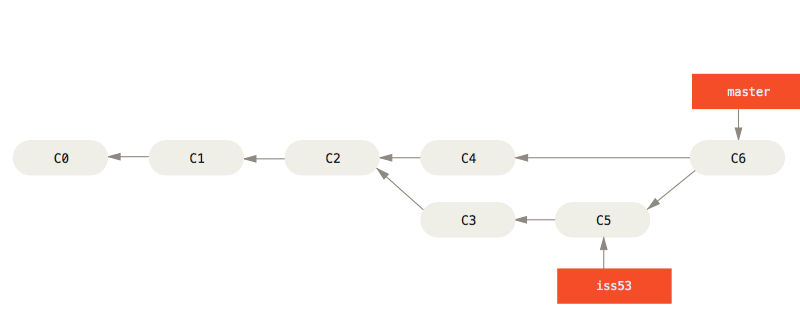
\includegraphics{static/timeline.png}\\
Source: https://git-scm.com/book/en/v2

    The git version control system can be thought of as a iterative workflow
where paper documents move between various places: - The modified state:
The document is on our desk before us and we edit (write) it. - Staged:
When our task on the document is done or we have to work on sth else, we
put the file into a shelf that has a label ``Keep'' on it. It can be
thought of as a stash of documents that we need to keep within reach but
are not actively working on it. From that stash, we can easily pull the
document back to our desk and continue working on it. - Committed: At
some point, we would like to take a snapshot of the document, so we can
re-open precisely the current state at a later point in time. In a paper
world, we would take the stash of documents to the copy machine, make a
copy from each document and put the copy into a file cabinet, tagged
with a date, our name, and a remark telling us what the change of this
copy with respect to the previous copy is. The original document is now
in a ``unmodified'' state (with respect to the last backup copy).

We then take the document back to our desk and continue working on it:
It is then again in the ``modified state''.

    \begin{figure}
\centering
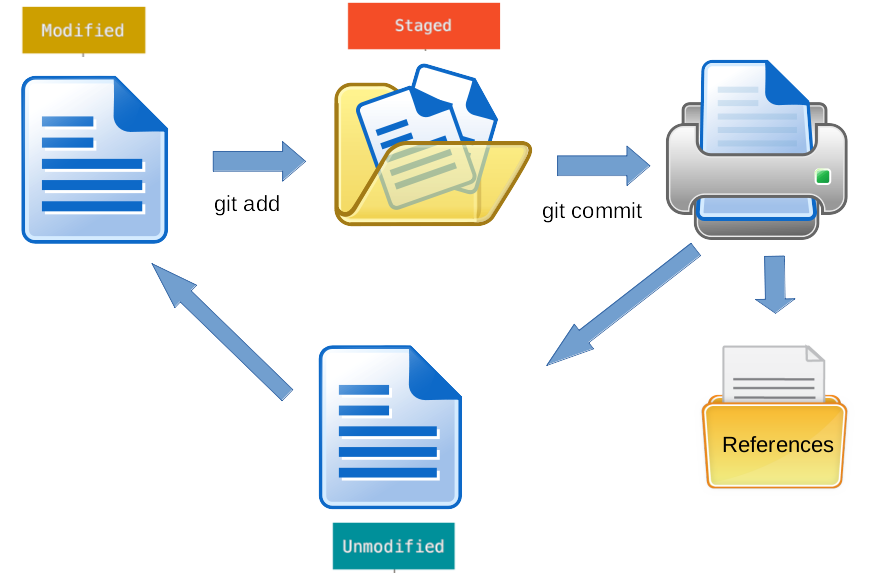
\includegraphics{static/track.png}
\caption{image.png}
\end{figure}

    \hypertarget{setting-up-git}{%
\section{Setting up git}\label{setting-up-git}}

Initially we need to set up git.

git keeps track of the entire history of a project. This does not only
mean keeping track of what was done but also who did it. So we start by
telling git who we are by running the following two commands:

\begin{verbatim}
$ git config --global user.name "Your Name"
$ git config --global user.email "Your Email"
\end{verbatim}

\textbf{Note} this is not data that is being collected by any cloud
service or similar. It just stays with your project.

\textbf{Windows} Note that all these commands work on the anaconda
prompt but if you want to use tab completion you can use the git bash
command line specifically for git.

Moreover, we are going to set \href{https://www.nano-editor.org}{Nano}
as the default editor for git. For unix you can use the following
command:

\begin{verbatim}
$ git config --global core.editor "nano"
\end{verbatim}

We are going to use Nano later in order to write a commit message.

    \hypertarget{initialising-a-git-repository}{%
\section{Initialising a git
repository}\label{initialising-a-git-repository}}

In order to demonstrate how version control with git works we are going
to use the \texttt{rsd-workshop} folder we created before.

We need tell git to start keeping an eye on this repository
(folder/project). While in the \texttt{rsd-workshop} directory type:

\begin{verbatim}
$ git init
\end{verbatim}

You should then see a message saying that you have successfully
initialized a git repository.

    \hypertarget{staging-and-committing-changes}{%
\section{Staging and committing
changes}\label{staging-and-committing-changes}}

To see the status of the repository we just initialized type:

\begin{verbatim}
$ git status
\end{verbatim}

We should see something like:

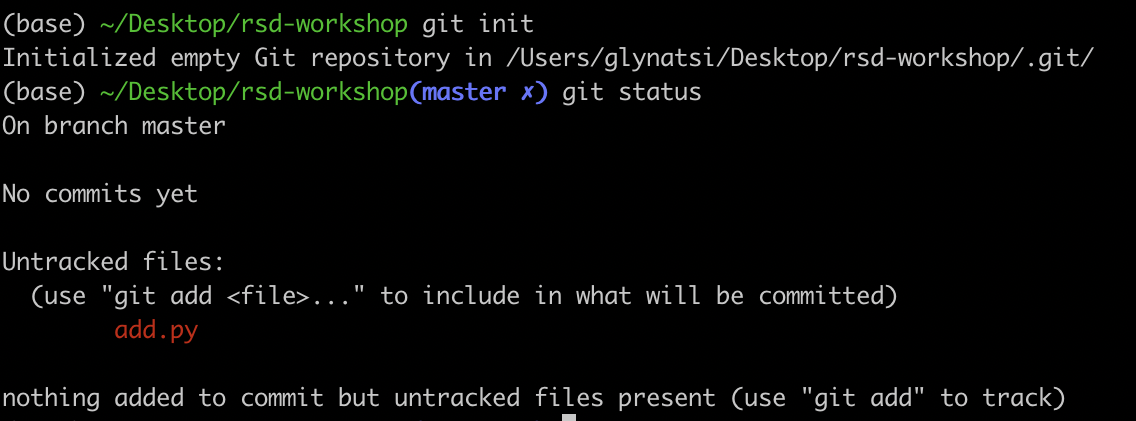
\includegraphics{static/git_status.png}

    There are various pieces of useful information here, first of all that
\texttt{addition.py}, \texttt{if-statement.py} and
\texttt{while-loops.py} are not currently tracked files.

We are now going to track the \texttt{addition.py} file:

\begin{verbatim}
$ git add addition.py
\end{verbatim}

If we run git status again we see:

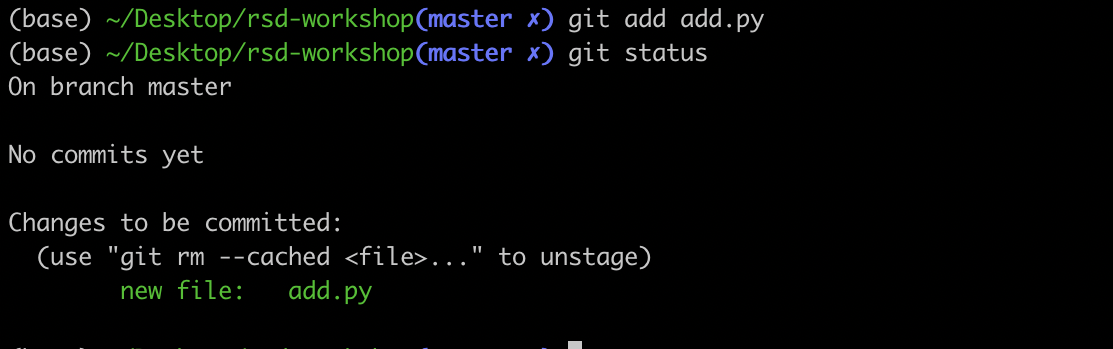
\includegraphics{static/git_status_after_add.png}

    We have propagated our file from the ``Untracked'' to the ``Staged''
status.\\

\includegraphics{static/staged.png}

    So the \texttt{addition.py} file is now ready to be ``committed''.

\begin{verbatim}
$ git commit
\end{verbatim}

When doing this, a text editor should open up prompting you to write
what is called a commit message. In our case the text editor that opens
is Nano.

For the purposes of using git Nano is more than a sufficient editor, all
you need to know how to do is:

\begin{itemize}
\tightlist
\item
  Write in Nano: just type;
\item
  Save in Nano: Ctrl + O;
\item
  Quit in Nano: Ctrl + X.
\end{itemize}

    Type the following as the first commit message:

\begin{verbatim}
Add addition script

Addition script contains a function which adds two numbers.
\end{verbatim}

save and exit.

git should confirm that you have successfully made your first commit.

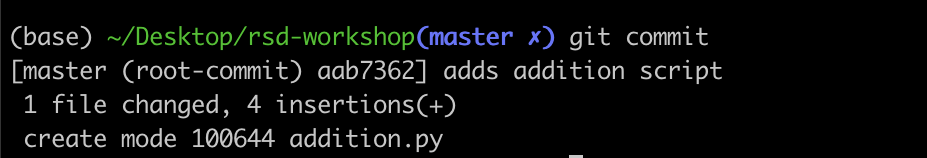
\includegraphics{static/git_commit.png}

    \textbf{Note} A commit message is made up of 2 main components:

\begin{verbatim}
<Title of the commit>

<Description of what was done>
\end{verbatim}

\begin{itemize}
\tightlist
\item
  The title should be a description in the form of ``if this commit is
  applied \texttt{\textless{}title\ of\ the\ commit\textgreater{}} will
  happen''. The convention is for this to be rather short and to the
  point.
\item
  The description can be as long as needed and should be a helpful
  explanation of what is happening.
\end{itemize}

A commit is a snapshot that git makes of your project, you should use
this at meaningful steps of the progress of a project.

    Now, our file is in the ``Unmodified'' state, because it is identical to
the \emph{copy} that we filed away to our ``file cabinet'' (the location
where git stores the snapshots).

\begin{figure}
\centering

\includegraphics{static/unmodified.png}
\caption{image.png}
\end{figure}

    \hypertarget{ignoring-files}{%
\section{Ignoring files}\label{ignoring-files}}

There are still two files in the repository that are currently not being
tracted. These are \texttt{if-statement.py} and \texttt{while-loops.py}.

We do not want to keep tract of those files as they are not related to
our project.

To tell git to ignore these files we will add them to a blank file
entitled \texttt{.gitignore}.

Open your editor and open a new file
(\texttt{File\ \textgreater{}\ New\ file}) and type:

\begin{verbatim}
if-statement.py
while-loops.py
\end{verbatim}

Save that file as \texttt{.gitignore} and then run:

\begin{verbatim}
$ git status 
\end{verbatim}

We see now that \texttt{git} is ignoring those 2 files but is aware of
the \texttt{.gitignore} file.

Let us add and commit that file:

\begin{verbatim}
$ git add .gigignore
$ git commit
\end{verbatim}

Use \texttt{Add\ .gitignore} as the commit message.

    Now if we run \texttt{git\ status}, we see a message saying that
everything in our repository is tracked and up to date.

    \hypertarget{tracking-changes-to-files} \DecValTok{2} \OperatorTok{==} \DecValTok{0} \KeywordTok{and}\NormalTok{ b }\OperatorTok{\%} \DecValTok{2} \OperatorTok{==} \DecValTok{0}\NormalTok{:}
        \ControlFlowTok{return}\NormalTok{ a }\OperatorTok{+}\NormalTok{ b}
    \ControlFlowTok{else}\NormalTok{:}
        \BuiltInTok{print}\NormalTok{(}\StringTok{"Please use even numbers."}\NormalTok{)}
    
\BuiltInTok{print}\NormalTok{(add\_two\_even\_numbers(}\DecValTok{4}\NormalTok{, }\DecValTok{6}\NormalTok{))}
\end{Highlighting}
\end{Shaded}

Save your file and then run:

\begin{verbatim}
$ git status
\end{verbatim}

We now see that git is aware of a change to our file:

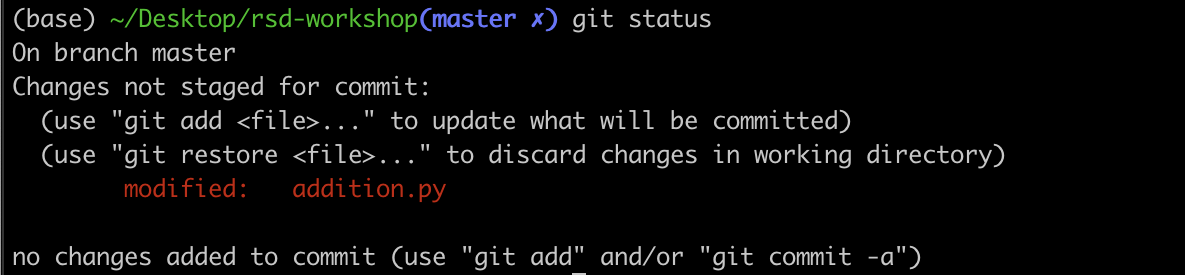
\includegraphics{static/modified.png}

    Our file is now in the modified state, as \texttt{git\ status} will tell
us.

\begin{figure}
\centering

\includegraphics{static/to_modified.png}
\caption{image.png}
\end{figure}

    To see what has been modified you need to type:

\begin{verbatim}
$ git diff addition
\end{verbatim}

and press \texttt{q} to exit.

To ``stage'' the file for a commit we use git add again:

\begin{verbatim}
$ git add addition
\end{verbatim}

Now let us commit:

\begin{verbatim}
$ git commit
\end{verbatim}

With the following commit message:

\begin{verbatim}
Change add two numbers function to add two even numbers
\end{verbatim}

Finally, we can check the status: git status to confirm that everything
has been done correctly.

    \hypertarget{exploring-history}{%
\section{Exploring history}\label{exploring-history}}

    \texttt{git} allows us to see the history of a project and in some cases
even change it. To view the history of a repository type:

\begin{verbatim}
$ git log
\end{verbatim}

This displays the full log of the project:

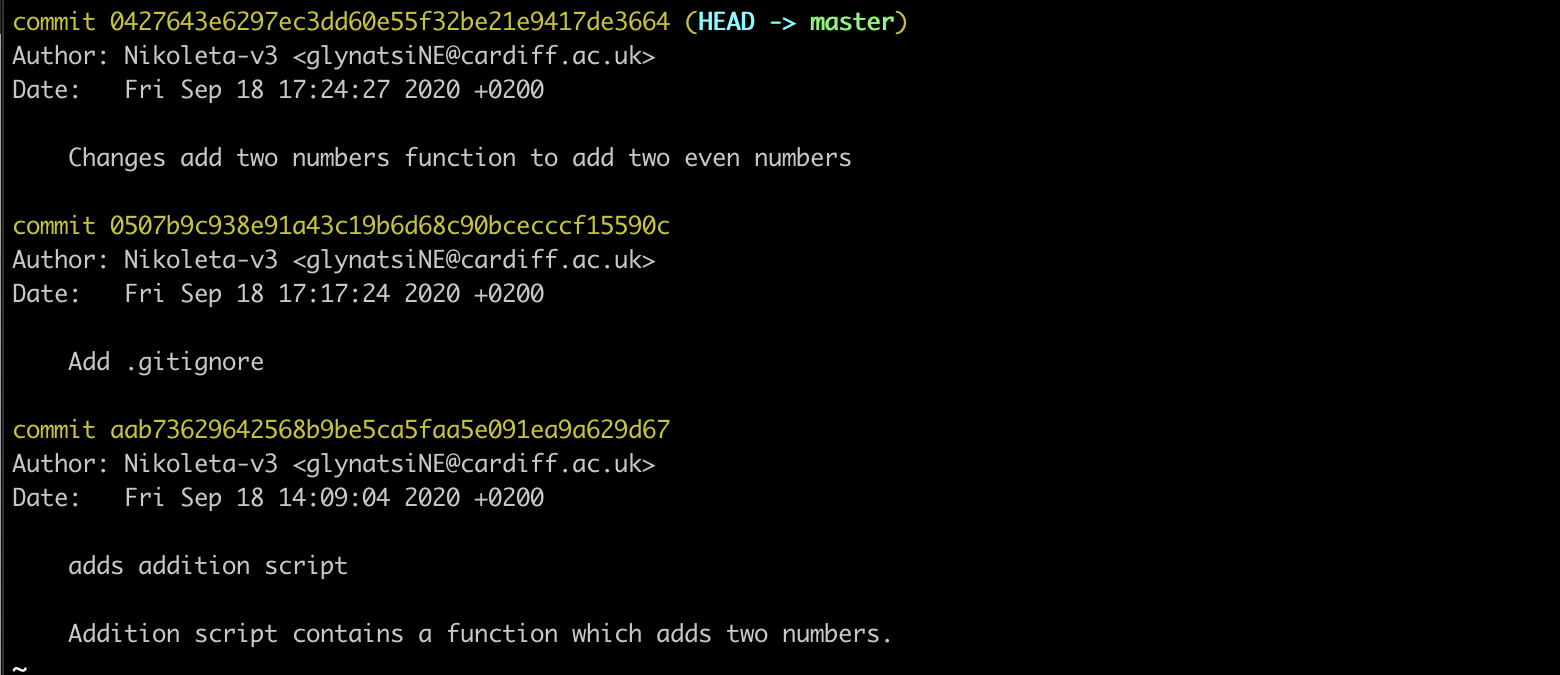
\includegraphics{static/git_log.png}

We see that there are 3 commits there, each with a seemingly random set
of numbers and characters. This set of characters is called a ``hash''.

The first commit with title \texttt{adds\ addition\ script} has hash:
aab73629642568b9be5ca5faa5e091ea9a629d67.

\textbf{Note} that on your machines this hash will be different, in fact
every hash is mathematically guaranteed to be unique, thus it is
uniquely assigned to the changes made.

Hashes can be very useful but we are not going to cover their many uses
in this workshop.

    \hypertarget{creating-branches}{%
\section{Creating branches}\label{creating-branches}}

The final part that we will cover in Day I is creating branches.
Branches allow us to work in parallel which is very important when
developing software, and also when we do research.

    When typing \texttt{git\ status} we have seen that one piece of
information regularly given was:

\begin{verbatim}
On branch master
\end{verbatim}

This is telling us which branch of ``history'' we are currently on. We
can view all branches with the command:

\begin{verbatim}
$ git branch
\end{verbatim}

This shows:

\begin{verbatim}
* master
\end{verbatim}

So currently there is only one branch called master. Let us create a new
branch called \texttt{implement-add-odd-numbers}:

\begin{verbatim}
$ git branch implement-add-odd-numbers
\end{verbatim}

When we now type \texttt{git\ branch} we see that 2 branches exist but
the active branch is indicated by *:

\begin{verbatim}
implement-add-odd-numbers
* master
\end{verbatim}

To move to this new branch the command is:

\begin{verbatim}
$ git checkout implement-add-odd-numbers
\end{verbatim}

Run \texttt{git\ branch} and then \texttt{git\ status} to see how this
has worked.

    While we are on this branch we are going to add a new function in the
\texttt{addition.py} and that is a function that adds two odd numbers.

Add the following code to \texttt{addition.py}:

\begin{Shaded}
\begin{Highlighting}[]
\KeywordTok{def}\NormalTok{ add\_two\_odd\_numbers(a, b):}
    \ControlFlowTok{if}\NormalTok{ a }\OperatorTok{\%} \DecValTok{2} \OperatorTok{!=} \DecValTok{0} \KeywordTok{and}\NormalTok{ b }\OperatorTok{\%} \DecValTok{2} \OperatorTok{!=} \DecValTok{0}\NormalTok{:}
        \ControlFlowTok{return}\NormalTok{ a }\OperatorTok{+}\NormalTok{ b}
    \BuiltInTok{print}\NormalTok{(}\StringTok{"Please use odd numbers."}\NormalTok{)}

\BuiltInTok{print}\NormalTok{(add\_two\_odd\_numbers(}\DecValTok{1}\NormalTok{, }\DecValTok{3}\NormalTok{))}
\end{Highlighting}
\end{Shaded}

    Let us add and commit this:

\begin{verbatim}
$ git add addition
$ git commit 
\end{verbatim}

Commit message:

\begin{verbatim}
Implement function for adding odd numbers
\end{verbatim}

    Let us now return to the master branch.

\begin{verbatim}
$ git checkout master
\end{verbatim}

If you open the file \texttt{addition.py} you will see that the latest
change is not there. That is because this change was done in a different
branch.

Branches allow us to bring work from different people done in parallel
and merged them to the main branch of the repository. This can be done
locally using \texttt{git} and also on the cloud using GitHub. This is
demonstrated in the material of Day II in the GitHub example.

    \hypertarget{time-travel-checking-out-a-previous-commit}{%
\subsection{Time travel: Checking out a (previous)
commit}\label{time-travel-checking-out-a-previous-commit}}

    The \texttt{git\ checkout} commands allows us to revert our file(s) to a
state from an earlier commit. Find the commit hash to revert to from
\texttt{git\ log} first. Highlight the hash and copy it (Ctrl-C). Then
paste into the \texttt{git\ checkout} command. It's actually sufficient
to take only the first 8 characters from the hash.

    \begin{verbatim}
$ git checkout fbb2cd03
\end{verbatim}

    The message about ``detached HEAD'' means that our file(s) have now
reverted to a state from an earlier commit. Any changes to our files
would not be commited directy back to our branch (more about branches
further below).

    The history reported by \texttt{git\ log} now contains only the commits
before the checked out commit as you can see by running

\begin{verbatim}
$ git log
\end{verbatim}

    \hypertarget{check-out-the-tip-of-the-branch-aka-head}{%
\subsection{Check out the tip of the branch (aka
HEAD)}\label{check-out-the-tip-of-the-branch-aka-head}}

    To go back to the ``tip of the branch'' (the state where we left from
before checking out an earlier commit) we run

    \begin{verbatim}
$ git checkout master
\end{verbatim}

    \begin{verbatim}
$ git status
\end{verbatim}

    \begin{verbatim}
$ git log
\end{verbatim}

    \hypertarget{merging-locally}{%
\subsubsection{Merging locally}\label{merging-locally}}

The \texttt{git\ merge} command integrates changes from a branch into
the currently checked out branch. Before merging, make sure to have
checked out the target branch. In our example we merge changes from the
``implement-add-odd-numbers'' branch into the ``master'' branch.

    \begin{verbatim}
$ git checkout master

Switched to branch 'master'
\end{verbatim}

    Now use the \texttt{git\ merge} command to bring in the changes from the
``implement-add-odd-numbers'' branch. It is good practice to always
append the \texttt{-\/-no-ff} flag to \texttt{git\ merge} to create a
dedicated merge commit. In this way one can later identify changes in
the code that are a result from a merge.

    \begin{verbatim}
$ git merge implement-add-odd-numbers --no-ff -m "Merge implement-add-odd-numbers"
\end{verbatim}

    Let's now look at our history. I will append some flags to
\texttt{git\ log} here that will visualize the tree-like structure of
our history:

    \begin{verbatim}
$ git log --pretty=oneline --graph --abbrev-commit
\end{verbatim}

    \hypertarget{delete-feature-branch}{%
\subsubsection{Delete feature branch}\label{delete-feature-branch}}

If we are certain that the feature branch \texttt{iss53} will no longer
be used, we can delete it:

    \begin{verbatim}
$ git branch -D implement-add-odd-numbers
\end{verbatim}

    \texttt{git\ branch} will tell us that master is now our only branch
again.

    \begin{verbatim}
$ git branch
\end{verbatim}


    % Add a bibliography block to the postdoc
    
    
    
\end{document}
